%%% LaTeX Template: Article/Thesis/etc. with colored headings and special fonts
%%%
%%% Source: http://www.howtotex.com/
%%% Feel free to distribute this template, but please keep to referal to http://www.howtotex.com/ here.
%%% February 2011
%%%
%%% Modified January 2016 by CDM

%%%  Preamble
\documentclass[11pt,letterpaper]{article}
\usepackage[margin=1.0in]{geometry}
\usepackage[T1]{fontenc}
\usepackage[bitstream-charter]{mathdesign}
\usepackage[latin1]{inputenc}					
\usepackage{amsmath}						
\usepackage{xcolor}
\usepackage{cite}
\usepackage{hyphenat}
\usepackage{graphicx}
\usepackage{float}
\usepackage{subfigure}
\usepackage{sectsty}
\usepackage[compact]{titlesec} 
\usepackage[tablegrid]{vhistory}
\allsectionsfont{\color{accentcolor}\scshape\selectfont}

%%% Definitions
\definecolor{accentcolor}{rgb}{0.0,0.0,0.5} 
\newcommand{\teamname}{VibeTracked}
\newcommand{\productname}{Cerberus}
\newcommand{\coursename}{CSE 4316: Senior Design I}
\newcommand{\semester}{Fall 2021}
\newcommand{\docname}{Architectural Design Specification}
\newcommand{\department}{Department of Computer Science \& Engineering}
\newcommand{\university}{The University of Texas at Arlington}
\newcommand{\authors}{Katie Baumann \\ Matthew Blount \\ Xavier Holliday \\ Vinson Mach \\ Lauren Skinner \\ Paul Zhi}

%%% Headers and footers
\usepackage{fancyhdr}
	\pagestyle{fancy}						% Enabling the custom headers/footers
\usepackage{lastpage}	
	% Header (empty)
	\lhead{}
	\chead{}
	\rhead{}
	% Footer
	\lfoot{\footnotesize \teamname \ - \semester}
	\cfoot{}
	\rfoot{\footnotesize page \thepage\ of \pageref{LastPage}}	% "Page 1 of 2"
	\renewcommand{\headrulewidth}{0.0pt}
	\renewcommand{\footrulewidth}{0.4pt}

%%% Change the abstract environment
\usepackage[runin]{abstract}			% runin option for a run-in title
%\setlength\absleftindent{30pt}			% left margin
%\setlength\absrightindent{30pt}		% right margin
\abslabeldelim{\quad}	
\setlength{\abstitleskip}{-10pt}
\renewcommand{\abstractname}{}
\renewcommand{\abstracttextfont}{\color{accentcolor} \small \slshape}	% slanted text

%%% Start of the document
\begin{document}

%%% Cover sheet
{\centering \huge \color{accentcolor} \sc \textbf{\department \\ \university} \par}
\vspace{1 in}
{\centering \huge \color{accentcolor} \sc \textbf{\docname \\ \coursename \\ \semester} \par}
\vspace{0.5 in}
\begin{figure}[h!]
	\centering
   	
\includegraphics[width=0.60\textwidth]{images/vibetracked-logo.png}
\end{figure}
\vspace{0.5 in}
{\centering \huge \color{accentcolor} \sc \textbf{\teamname \\ \productname} \par}
\vspace{0.5 in}
{\centering \large \sc \textbf{\authors} \par}
\newpage


%\vspace{1 in}
%\centerline{January 13th, 2012}
%\newpage

%%% Revision History
\begin{versionhistory}
  	\vhEntry{0.1}{10.29.2021}{VM}{document creation}
  	\vhEntry{1.0}{11.15.2021}{KB|MB|XH|VM|LS|PZ}{first draft completion}
\end{versionhistory}
\newpage

%%% Table of contents
\setcounter{tocdepth}{2}
\tableofcontents
\newpage

%%% List of figures and tables (optional)
\listoffigures
\listoftables
\newpage

%%% Document sections
\section{Introduction}
Your introduction should provide a brief overview of the product concept and a reference to the requirement specification and architectural design documents in 1 or 2 paragraphs. The purpose is to provide the reader with the location of relevant background material that lead to the design details presented in this document.

\newpage
\section{System Overview}
Explain, at a high level, how you will implement a solution to the problem. Include a diagram of major components to the system (not a full architectural design, but a high level overview of the major system components and how a user or external system might interface). Avoid specific implementation details (operating system, programming languages, etc.). This section should occupy at least 1 full page.
\newpage
\section{Subsystem Definitions \& Data Flow}
This section breaks down your layer abstraction to another level of detail. Here you grapically represent the logical subsytems that compose each layer and show the interactions/interfaces between those subsystems. A subsystem can be thought of as a programming unit that implements one of the major functions of the layer. It, therefore, has data elements that serve as source/sinks for other subsystems. The logical data elements that flow between subsystems need to be explicitly defined at this point, beginning with a data flow-like diagram based on the block diagram.

\begin{figure}[h!]
	\centering
 	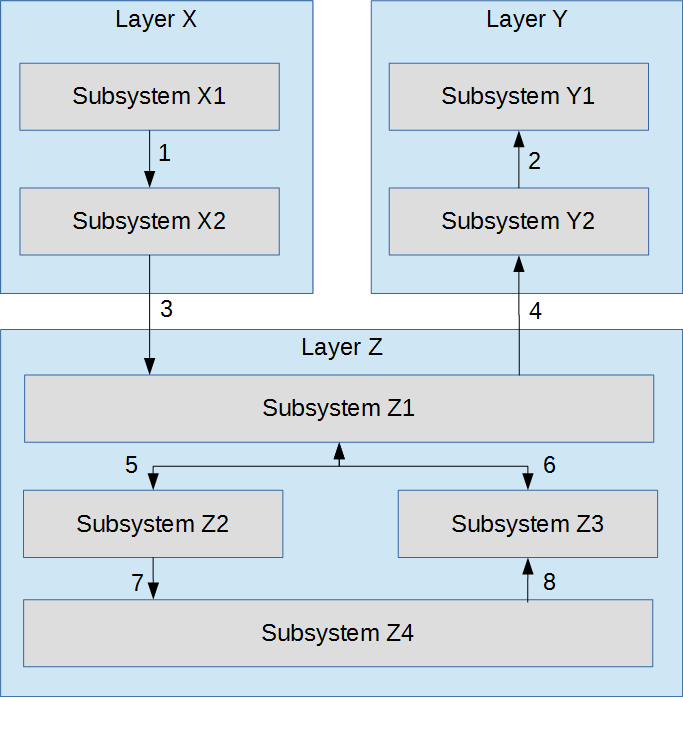
\includegraphics[width=\textwidth]{images/data_flow}
 \caption{A simple data flow diagram}
\end{figure}

\newpage
\section{Power Management Layer Subsystems}
In the section, the power management layer is described in greater detail in terms of its subsystems.

\subsection{Charging}
%This section should be a general description of a particular subsystem for the given layer. For most subsystems, an extract of the architectural block diagram with data flows is useful. This should consist of the subsystem being described and those subsystems with which it communicates.

\begin{figure}[h!]
	\centering
 	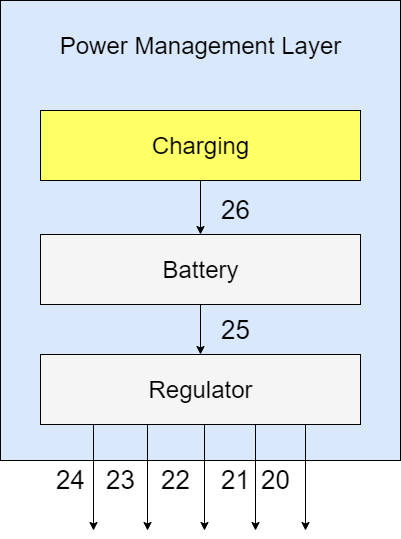
\includegraphics[width=0.60\textwidth]{images/PowerMgmtLayer_charging.drawio.png}
 \caption{Power Management Charging Subsystem diagram}
\end{figure}

\subsubsection{Assumptions}
%Any assumptions made in the definition of the subsystem should be listed and described. Pay particular attention to assumptions concerning interfaces and interactions with other layers.
The user has access to electricity and has the proper charging cable for the wristband.

\subsubsection{Responsibilities}
%Each of the responsibilities/features/functions/services of the subsystem as identified in the architectural summary must be expanded to more detailed responsibilities. These responsibilities form the basis for the identification of the finer-grained responsibilities of the layer's internal subsystems. Clearly describe what each subsystem does.
This subsystem is responsible for charging the wristband's battery. It must be able to charge the wristband within a reasonable time frame. It will take a USB-c cable that can be plugged into a USB outlet. 

\subsubsection{Subsystem Interfaces}
%Each of the inputs and outputs for the subsystem are defined here. Create a table with an entry for each labelled interface that connects to this subsystem. For each entry, describe any incoming and outgoing data elements will pass through this interface.

\begin{table}[H]
\caption{Charging Interfaces}
\begin{center}
\begin{tabular}{|l|l|l|l|}
    \hline
    ID & Description & Input & Output \\ \hline
    26 & Charging to battery & N/A & Voltage \\ \hline
\end{tabular}
\end{center}
\end{table}

\subsection{Battery}

\begin{figure}[h!]
	\centering
 	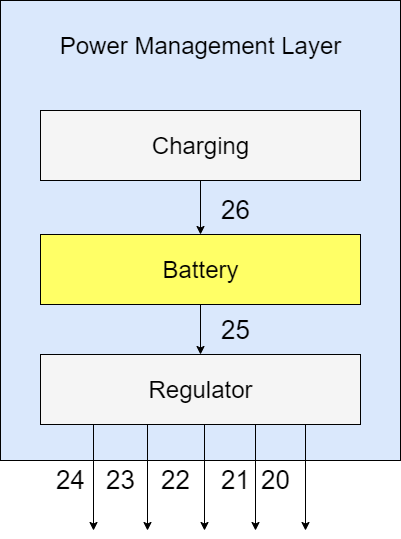
\includegraphics[width=0.60\textwidth]{images/PowerMgmtLayer_battery.drawio.png}
 \caption{Power Management Battery Subsystem diagram}
\end{figure}

\subsubsection{Assumptions}
%Any assumptions made in the definition of the subsystem should be listed and described. Pay particular attention to assumptions concerning interfaces and interactions with other layers.
The user has access to electricity to charge the battery. The battery is working properly and not damaged. 

\subsubsection{Responsibilities}
%Each of the responsibilities/features/functions/services of the subsystem as identified in the architectural summary must be expanded to more detailed responsibilities. These responsibilities form the basis for the identification of the finer-grained responsibilities of the layer's internal subsystems. Clearly describe what each subsystem does.
This subsystem is responsible for powering the all the wristband components. It must be strong enough to power all the wristband components. The battery must be long lasting to prevent the user from having to charge it constantly. 

\subsubsection{Subsystem Interfaces}

\begin{table}[H]
\caption{Battery Interfaces}
\begin{center}
\begin{tabular}{|l|l|l|l|}
    \hline
    ID & Description & Input & Output \\ \hline
    25 & Battery to Regulator  & Voltage  & Power (W)  \\ \hline
\end{tabular}
\end{center}
\end{table}

\subsection{Regulator}

\begin{figure}[h!]
	\centering
 	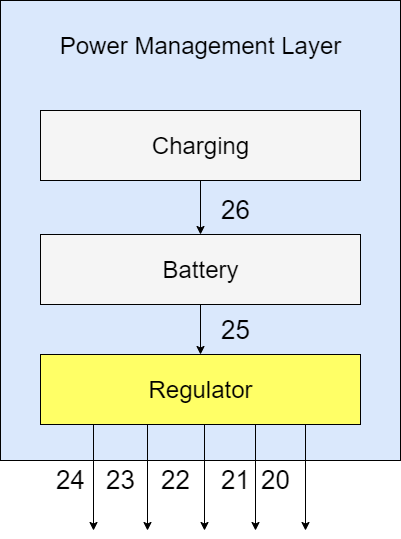
\includegraphics[width=0.60\textwidth]{images/PowerMgmtLayer_regulator.drawio.png}
 \caption{Power Management Regulator Subsystem diagram}
\end{figure}

\subsubsection{Assumptions}
%Any assumptions made in the definition of the subsystem should be listed and described. Pay particular attention to assumptions concerning interfaces and interactions with other layers.
The wristband is properly charged and working. The wristband is not damaged or malfunctioning. 

\subsubsection{Responsibilities}
%Each of the responsibilities/features/functions/services of the subsystem as identified in the architectural summary must be expanded to more detailed responsibilities. These responsibilities form the basis for the identification of the finer-grained responsibilities of the layer's internal subsystems. Clearly describe what each subsystem does.
This subsystem is responsible for regulating the power coming from the battery to the other wristband components. It must delegate enough power to each component so the wristband can function properly. It must not drain the battery too fast.

\subsubsection{Subsystem Interfaces}

\begin{table}[H]
\caption{Regulator interfaces}
\begin{center}
\begin{tabular}{|l|l|l|l|}
    \hline
    ID & Description & Inputs & Outputs \\ \hline
    24 & Power to Bluetooth Module & Power (W) & Power (W) \\ \hline
    23 & Power to Micro-Controller & Power (W) & Power (W) \\ \hline
    22 & Power to Vibration Module & Power (W) & Power (W) \\ \hline
    21 & Power to Audio Sensor & Power (W) & Power (W) \\ \hline
    20 & Power to LED lights & Power (W) & Power (W) \\ \hline
    % I think I am supposed to put all the wristband components here
\end{tabular}
\end{center}
\end{table}

\newpage
\section{Wristband Layer Subsystems}
In the section, the wristband layer is described in greater detail in terms of its subsystems.
% In this section, the layer is described in some detail in terms of its specific subsystems. Describe each of the layers and its subsystems in a separate chapter/major subsection of this document. The content of each subsystem description should be similar. Include in this section any special considerations and/or trade-offs considered for the approach you have chosen.


\subsection{Micro-controller}
This subsystem is responsible for controlling the overall functioning of the device.

\begin{figure}[h!]
	\centering
 	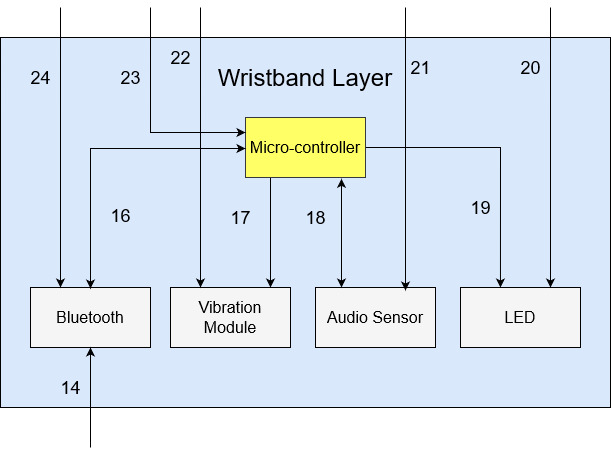
\includegraphics[width=0.60\textwidth]{images/wristband-micro.jpg}
 \caption{Wristband Micro-controller Subsystem diagram}
\end{figure}

\subsubsection{Assumptions}
It is assumed that all modules are properly connected and working. It is also assumed that there is power in the system.

\subsubsection{Responsibilities}
The micro-controller is connected to the Bluetooth, vibration, audio sensor, and LED modules. Once a Bluetooth signal is received to vibrate, the micro-controller sends a signal to the vibration module to vibrate in a specific pattern. Additionally, once the audio sensor detects a certain decibel level, the micro-controller sends a signal to the LED to be a certain color.

\subsubsection{Subsystem Interfaces}

\begin {table}[H]
\caption {Micro-Controller interfaces} 
\begin{center}
    \begin{tabular}{ | p{1cm} | p{6cm} | p{3cm} | p{3cm} |}
    \hline
    ID & Description & Inputs & Outputs \\ \hline
    16 & Bluetooth - Micro-Controller & Instructions for Vibrations & Signals \& Instructions to Operate \\ \hline
    17 & Vibration Module - Micro-Controller & N/A & Signals to Vibrate \\ \hline
    18 & Audio Sensor - Micro-Controller & Decibel Levels & Signals to Operate \\ \hline
    19 & LED - Micro-Controller & N/A & Signals \& Colors to Light \\ \hline
    23 & Power - Micro-Controller & Power (W) & N/A \\ \hline
%    \#xx & Description of the interface/bus & \pbox{3cm}{input 1 \\ input 2} & \pbox{3cm}{output 1}  \\ \hline
    %\#xx & Description of the interface/bus & \pbox{3cm}{N/A} & \pbox{3cm}{output 1}  \\ \hline
    \end{tabular}
\end{center}
\end{table}

\subsection{Bluetooth}
The Bluetooth subsystem is responsible for connecting to the user's phone and receiving signals via the Cerberus app.

\begin{figure}[h!]
	\centering
 	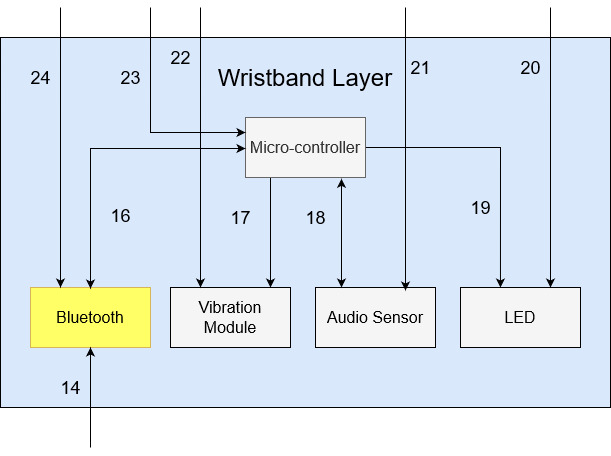
\includegraphics[width=0.60\textwidth]{images/wristband-bluetooth.jpg}
 \caption{Wristband Bluetooth Subsystem diagram}
\end{figure}

\subsubsection{Assumptions}
It is assumed that the Bluetooth module is functioning properly. It is also assumed that wristband is charged and the Bluetooth module is receiving power from the power layer.

\subsubsection{Responsibilities}
The Bluetooth module must be able to connect to devices capable of receiving Bluetooth signals. Upon connection, it must stay connected to the device. Once connected to the device, when it receives information from the Cerberus app such as notifications and vibration signals, it will send the information to the micro-controller.

\subsubsection{Subsystem Interfaces}

\begin {table}[H]
\caption {Bluetooth interfaces} 
\begin{center}
    \begin{tabular}{ | p{1cm} | p{6cm} | p{3cm} | p{3cm} |}
    \hline
    ID & Description & Inputs & Outputs \\ \hline
    14 & Bluetooth to Phone App & Vibration Instructions & Connectivity Signals \\ \hline
    16 & Bluetooth - Micro-controller & Instructions & Signals to Vibrate \\ \hline
    24 & Power to Bluetooth & Power (W) & N/A \\ \hline
    %\#xx & Description of the interface/bus & \pbox{3cm}{input 1 \\ input 2} & \pbox{3cm}{output 1}  \\ \hline
    %\#xx & Description of the interface/bus & \pbox{3cm}{N/A} & \pbox{3cm}{output 1}  \\ \hline
    \end{tabular}
\end{center}
\end{table}

\subsection{Audio Sensor}
The audio sensor detects decibel levels so the LED can be changed to a specific color.

\begin{figure}[h!]
	\centering
 	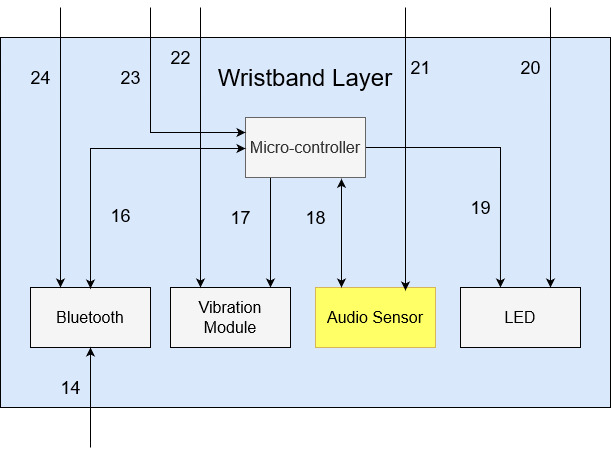
\includegraphics[width=0.60\textwidth]{images/wristband-audio.jpg}
 \caption{Wristband Audio Sensor Subsystem diagram}
\end{figure}

\subsubsection{Assumptions}
It is assumed that the module is functional and there is power in the power layer.

\subsubsection{Responsibilities}
The audio sensor is responsible for detecting the decibel level in the area the sensor is in. It is responsible for sending the audio readings to the micro-controller.

\subsubsection{Subsystem Interfaces}

\begin {table}[H]
\caption {Audio Sensor interfaces} 
\begin{center}
    \begin{tabular}{ | p{1cm} | p{6cm} | p{3cm} | p{3cm} |}
    \hline
    ID & Description & Inputs & Outputs \\ \hline
    18 & Bluetooth - Micro-controller & Setup Instructions & Audio \\ \hline
    21 & Power to Audio Sensor & Power (W) &  N/A \\ \hline
    %\#xx & Description of the interface/bus & \pbox{3cm}{input 1 \\ input 2} & \pbox{3cm}{output 1}  \\ \hline
    %\#xx & Description of the interface/bus & \pbox{3cm}{N/A} & \pbox{3cm}{output 1}  \\ \hline
    \end{tabular}
\end{center}
\end{table}

\subsection{LED}
This subsystem lights up according to the decibel level in the room.

\begin{figure}[h!]
	\centering
 	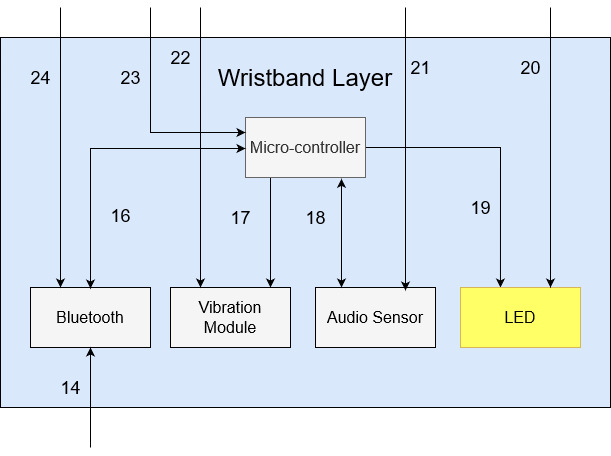
\includegraphics[width=0.60\textwidth]{images/wristband-led.jpg}
 \caption{Wristband Bluetooth Subsystem diagram}
\end{figure}

\subsubsection{Assumptions}
It is assumed that there is power in the system. It is also assumed that the audio sensor subsystem is operating properly.

\subsubsection{Responsibilities}
This subsystem is responsible for receiving the room's current decibel level from the micro-controller. It then lights up red if the room is loud, yellow if some noise, but not much, and green if quiet.

\subsubsection{Subsystem Interfaces}

\begin {table}[H]
\caption {LED interfaces} 
\begin{center}
    \begin{tabular}{ | p{1cm} | p{6cm} | p{3cm} | p{3cm} |}
    \hline
    ID & Description & Inputs & Outputs \\ \hline
    19 & Power to LEDs & Power (W) &  N/A \\ \hline
    20 & LED - Micro-controller & Instructions & N/A \\ \hline
    %\#xx & Description of the interface/bus & \pbox{3cm}{input 1 \\ input 2} & \pbox{3cm}{output 1}  \\ \hline
    %\#xx & Description of the interface/bus & \pbox{3cm}{N/A} & \pbox{3cm}{output 1}  \\ \hline
    \end{tabular}
\end{center}
\end{table}

\subsection{Vibration Module}
This subsystem is responsible for vibrating various patterns depending on what information is received from the micro-controller.

\begin{figure}[h!]
	\centering
 	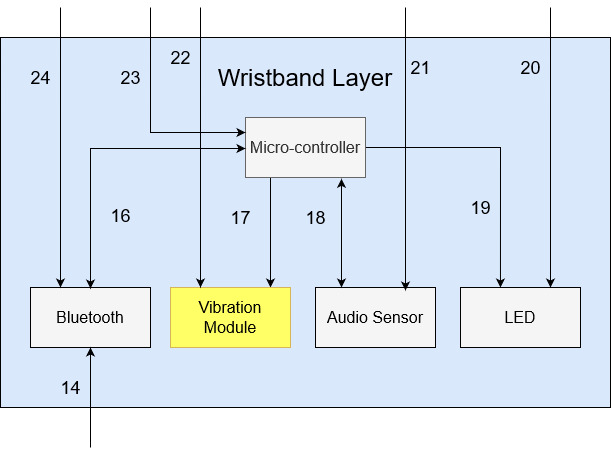
\includegraphics[width=0.60\textwidth]{images/wristband-vibration.jpg}
 \caption{Wristband Vibration Subsystem diagram}
\end{figure}

\subsubsection{Assumptions}
It is assumed that there is power in the system. It is also assumed that the Bluetooth module and micro-controller are functioning properly.

\subsubsection{Responsibilities}
This subsystem is responsible for receiving signals from the micro-controller to vibrate, causing the vibration motor to vibrate in specific patterns.

\subsubsection{Subsystem Interfaces}

\begin {table}[H]
\caption {Vibration Module interfaces} 
\begin{center}
    \begin{tabular}{ | p{1cm} | p{6cm} | p{3cm} | p{3cm} |}
    \hline
    ID & Description & Inputs & Outputs \\ \hline
    17 & Power to Vibration Motor & Power (W) &  N/A \\ \hline
    22 & Vibration Motor - Micro-controller & Instructions & N/A \\ \hline
    %\#xx & Description of the interface/bus & \pbox{3cm}{input 1 \\ input 2} & \pbox{3cm}{output 1}  \\ \hline
    %\#xx & Description of the interface/bus & \pbox{3cm}{N/A} & \pbox{3cm}{output 1}  \\ \hline
    \end{tabular}
\end{center}
\end{table}

\newpage
\section{Server Subsystems}

The Server Layer contains the notification and the database subsystems. The notification subsystem will handle the notifications that are pushed to the phone app and the database subsystem will handle the notification logs, account handling as well as the history logs. 

\subsection{Notifications}
This subsystem will handle the notifications that the phone app will receive from the server as well as the notifications received from various sensors. The notifications subsystem will work in tandem with the database subsystem to log notifications and push them to the user's phone app.

\begin{figure}[h!]
	\centering
 	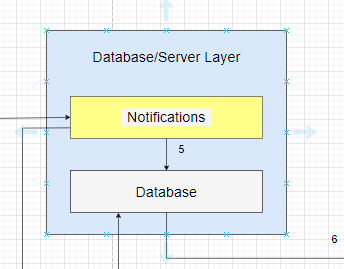
\includegraphics[width=0.60\textwidth]{images/Server_Layer1}
 \caption{Server Notifications Subsystem diagram}
\end{figure}

\subsubsection{Assumptions}
It is assumed that the user has setup their notification settings on the phone app as well as the server settings. 

\subsubsection{Responsibilities}
This subsystem will handle all notifications received from the various sensors and notifications to be sent to the user's phone app. 

\subsubsection{Subsystem Interfaces}

\begin {table}[H]
\caption {Notifications interfaces} 
\begin{center}
    \begin{tabular}{ | p{1cm} | p{6cm} | p{3cm} | p{3cm} |}
    \hline
    ID & Description & Inputs & Outputs \\ \hline
    4 & Notification Logs & Event signal from database & Notification Logs Page \\ \hline
    15 & Phone App Notifications & Event signal from database & Notification pushed to phone app \\ \hline
    \end{tabular}
\end{center}
\end{table}

\subsection{Database}
This subsystem will handle the user's login information, history logs, as well as the notification logs. The database subsystem will work in tandem with the notifications subsystem as well as the various sensors that are on the wristband layer.

\begin{figure}[h!]
	\centering
 	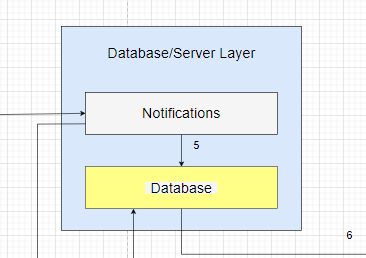
\includegraphics[width=0.60\textwidth]{images/Server_Layer2}
 \caption{Server Database Subsystem diagram}
\end{figure}

\subsubsection{Assumptions}
It is assumed that the database is connected to the phone app and the phone app will be able to communicate with the database. 

\subsubsection{Responsibilities}
This subsystem will handle all of the user's login information, history logs and the notification information. 

\subsubsection{Subsystem Interfaces}

\begin {table}[H]
\caption {Database interfaces} 
\begin{center}
    \begin{tabular}{ | p{1cm} | p{6cm} | p{3cm} | p{3cm} |}
    \hline
    ID & Description & Inputs & Outputs \\ \hline
    6 & Login information & User login information & Tokenized user login \\ \hline
    7 & History Logs & Event signal from various sensors & History Log Page \\ \hline
    \end{tabular}
\end{center}
\end{table}
\newpage
\section{Ring Base Subsystems}
%In this section, the layer is described in some detail in terms of its specific subsystems. Describe each of the layers and its subsystems in a separate chapter/major subsection of this document. The content of each subsystem description should be similar. Include in this section any special considerations and/or trade-offs considered for the approach you have chosen.
In the section, the Ring System layer is described in greater detail in terms of its subsystems.

\subsection{Ring Station}
%This section should be a general description of a particular subsystem for the given layer. For most subsystems, an extract of the architectural block diagram with data flows is useful. This should consist of the subsystem being described and those subsystems with which it communicates.

\begin{figure}[h!]
	\centering
 	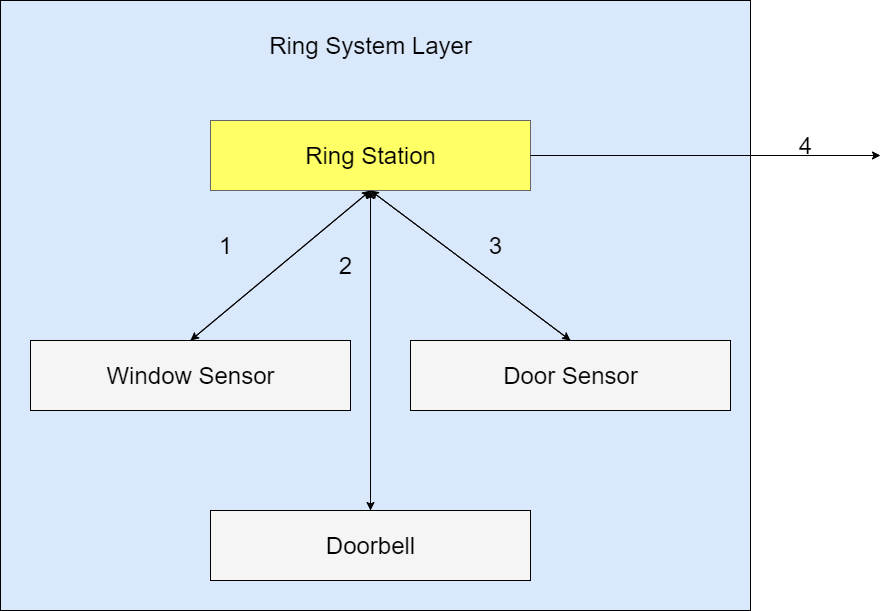
\includegraphics[width=0.60\textwidth]{images/RingLayer.drawio1.png}
 \caption{Ring Base Ring Station Subsystem diagram}
\end{figure}

\subsubsection{Assumptions}
Signals may be intercepted, or flags may be read from the ring doorbell system. We hope to use Ring to help receive signals either away from or outside of the house.

\subsubsection{Responsibilities}
The ring system must be responsible for picking up signals to alert the phone so that the wristband may vibrate.

\subsubsection{Subsystem Interfaces}

\begin {table}[H]
\caption {Ring Station interfaces} 
\begin{center}
    \begin{tabular}{ | p{1cm} | p{6cm} | p{3cm} | p{3cm} |}
    \hline
    ID & Description & Inputs & Outputs \\ \hline
    4 & Ring Station & signals from ring subsystems & notifications  \\ \hline
    \end{tabular}
\end{center}
\end{table}
\newpage

\subsection{Window Sensor}
%This section should be a general description of a particular subsystem for the given layer. For most subsystems, an extract of the architectural block diagram with data flows is useful. This should consist of the subsystem being described and those subsystems with which it communicates.

\begin{figure}[h!]
	\centering
 	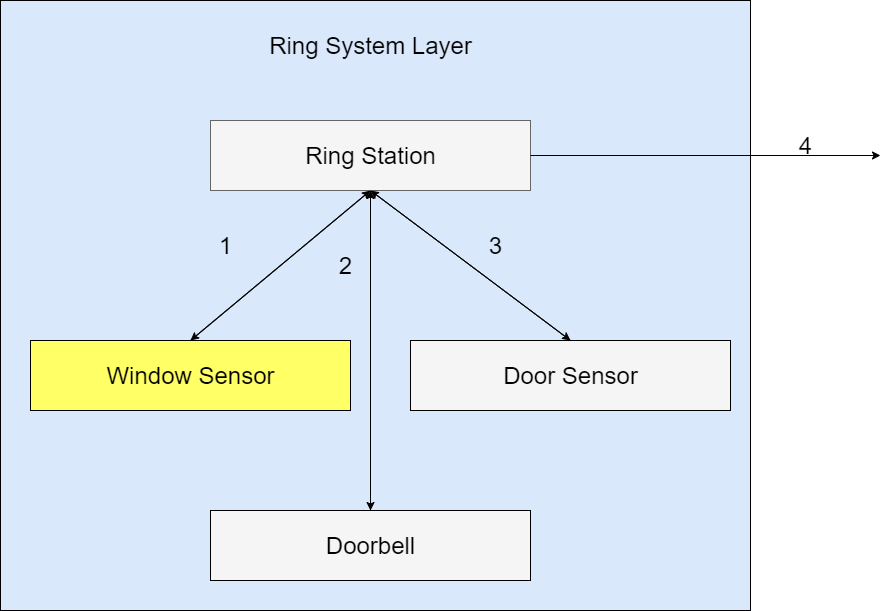
\includegraphics[width=0.60\textwidth]{images/RingLayer.drawio2.png}
 \caption{Ring Base Ring Station Subsystem diagram}
\end{figure}

\subsubsection{Assumptions}
Signals may be intercepted, or flags may be read from the ring doorbell system. We hope to use Ring to help receive signals either away from or outside of the house.

\subsubsection{Responsibilities}
The window sensor will detect if windows in the house are being opened. It will alert the Ring station of this detection.

\subsubsection{Subsystem Interfaces}

\begin {table}[H]
\caption {Window Sensor interfaces} 
\begin{center}
    \begin{tabular}{ | p{1cm} | p{6cm} | p{3cm} | p{3cm} |}
    \hline
    ID & Description & Inputs & Outputs \\ \hline
    2 & Window Sensor & Window Signal Received & Window Flag passed  \\ \hline

    \end{tabular}
\end{center}
\end{table}

\subsection{Doorbell}
%This section should be a general description of a particular subsystem for the given layer. For most subsystems, an extract of the architectural block diagram with data flows is useful. This should consist of the subsystem being described and those subsystems with which it communicates.

\begin{figure}[h!]
	\centering
 	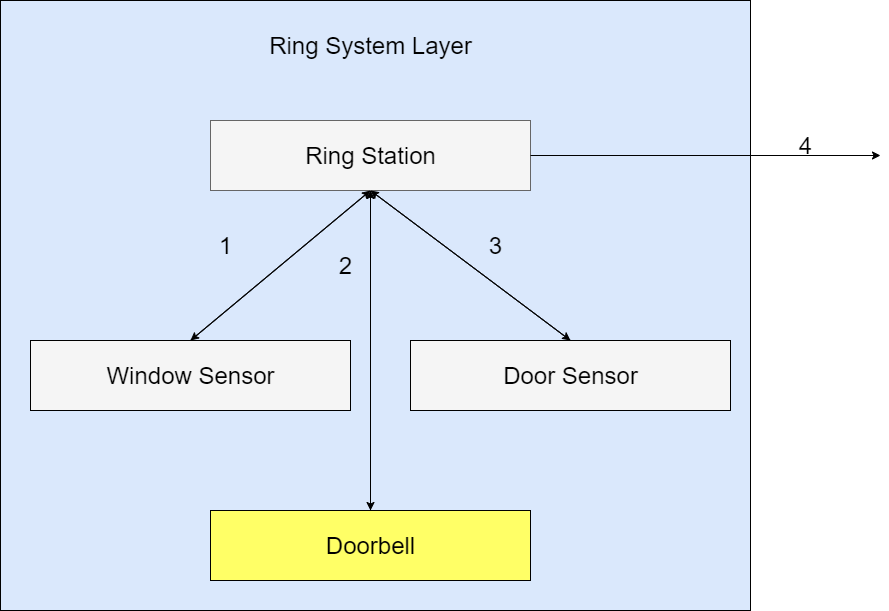
\includegraphics[width=0.60\textwidth]{images/RingLayer.drawio3.png}
 \caption{Ring Base Ring Station Subsystem diagram}
\end{figure}

\subsubsection{Assumptions}
Signals may be intercepted, or flags may be read from the ring doorbell system. We hope to use Ring to help receive signals either away from or outside of the house.

\subsubsection{Responsibilities}
The doorbell will detect the user of people at the door. It will alert the Ring station of this detection.

\subsubsection{Subsystem Interfaces}

\begin {table}[H]
\caption {Doorbell interfaces} 
\begin{center}
    \begin{tabular}{ | p{1cm} | p{6cm} | p{3cm} | p{3cm} |}
    \hline
    ID & Description & Inputs & Outputs \\ \hline
    1 & Doorbell & Ring Doorbell Signal received & Doorbell Flag passed  \\ \hline
    \end{tabular}
\end{center}
\end{table}

\subsection{Door Sensor}
%This section should be a general description of a particular subsystem for the given layer. For most subsystems, an extract of the architectural block diagram with data flows is useful. This should consist of the subsystem being described and those subsystems with which it communicates.

\begin{figure}[h!]
	\centering
 	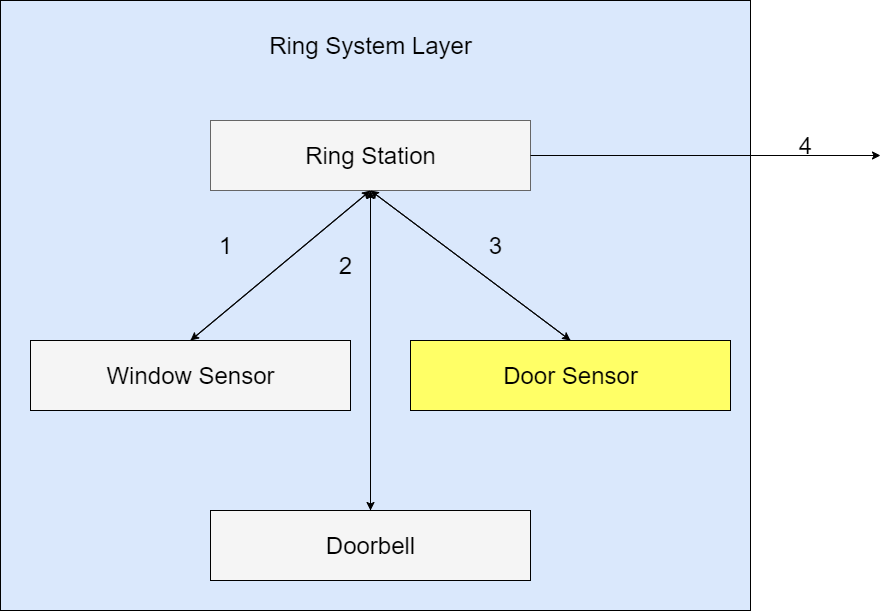
\includegraphics[width=0.60\textwidth]{images/RingLayer.drawio4.png}
 \caption{Ring Base Ring Station Subsystem diagram}
\end{figure}

\subsubsection{Assumptions}
Signals may be intercepted, or flags may be read from the ring doorbell system. We hope to use Ring to help receive signals either away from or outside of the house.

\subsubsection{Responsibilities}
The door sensor will detect if the door is being opened. It will alert the Ring station of this detection.

\subsubsection{Subsystem Interfaces}

\begin {table}[H]
\caption {Ring Station interfaces} 
\begin{center}
    \begin{tabular}{ | p{1cm} | p{6cm} | p{3cm} | p{3cm} |}
    \hline
    ID & Description & Inputs & Outputs \\ \hline
    3 & Door Sensor & Door Signal Received & Door Flag passed  \\ \hline
    \end{tabular}
\end{center}
\end{table}

\newpage
\section{Phone App Subsystems}
The phone app layer contains subsystems of Bluetooth, alert notification or history, notification setting, and vibration setting.

\subsection{Log in}
The text written through the app login ID and the information on the mobile phone will be uploaded to the web server and the corresponding value will be stored in the database system. 

\begin{figure}[h!]
	\centering
 	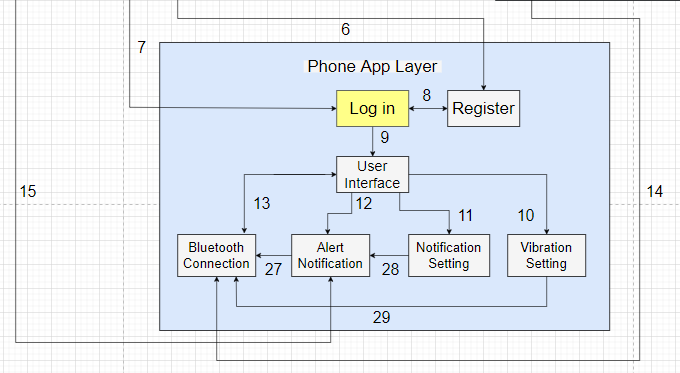
\includegraphics[width=0.60\textwidth]{images/phone_login.png}
 \caption{Phone App Layer diagram}
\end{figure}

\subsubsection{Assumptions}
The user has an android app downloaded on his/her phone and created an account.

\subsubsection{Responsibilities}
This subsystem is responsible for specifying a user and bringing information from the database.

\subsubsection{Subsystem Interfaces}
Each of the inputs and outputs for the subsystem are defined here. Create a table with an entry for each labelled interface that connects to this subsystem. For each entry, describe any incoming and outgoing data elements will pass through this interface.

\begin {table}[H]
\caption {Log in interfaces} 
\begin{center}
    \begin{tabular}{ | p{1cm} | p{6cm} | p{3cm} | p{3cm} |}
    \hline
    ID & Description & Inputs & Outputs \\ \hline
    #7 & From database & \pbox{Database information} & \pbox{User login information}  \\ \hline
    #9 & Login information & \pbox{User ID, User password} & \pbox{User wristband information}  \\ \hline
    #8 & To Registration page & \pbox{Click on the 'Register' button} & \pbox{Registration page}  \\ \hline
    \end{tabular}
\end{center}
\end{table}

\subsection{Register}
The register subsystem will hold new account information and store it in the database. The user’s email address will be the log-in ID and the system will ask the user to verify the email before proceeding.  

\begin{figure}[h!]
	\centering
 	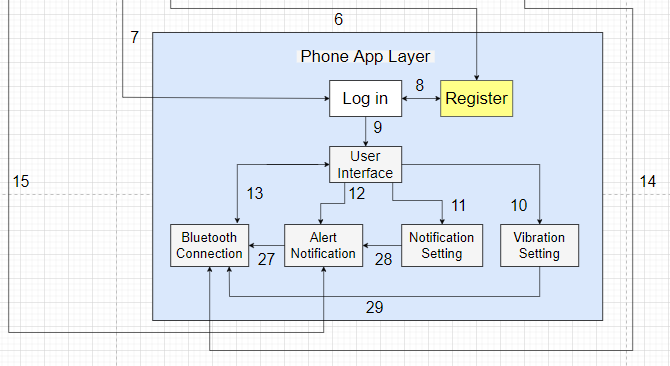
\includegraphics[width=0.60\textwidth]{images/phone_register.png}
 \caption{Phone App Layer diagram}
\end{figure}

\subsubsection{Assumptions}
The user has an android app downloaded on his/her phone and the app has access to the database.

\subsubsection{Responsibilities}
This subsystem is responsible for creating a new account and storing the information in the database so that the user is able to log in.

\subsubsection{Subsystem Interfaces}
Each of the inputs and outputs for the subsystem are defined here. Create a table with an entry for each labelled interface that connects to this subsystem. For each entry, describe any incoming and outgoing data elements will pass through this interface.

\begin {table}[H]
\caption {Register interfaces} 
\begin{center}
    \begin{tabular}{ | p{1cm} | p{6cm} | p{3cm} | p{3cm} |}
    \hline
    ID & Description & Inputs & Outputs \\ \hline
    #6 & User information & \pbox{Name, Email address, Password} & \pbox{App main page}  \\ \hline
    #8 & To previous page & \pbox{Click on the 'Back' button} & \pbox{Log in page}  \\ \hline
    \end{tabular}
\end{center}
\end{table}

\subsection{User interface}
The user interface subsystem will allow user to go to desire settings and make changes.   

\begin{figure}[h!]
	\centering
 	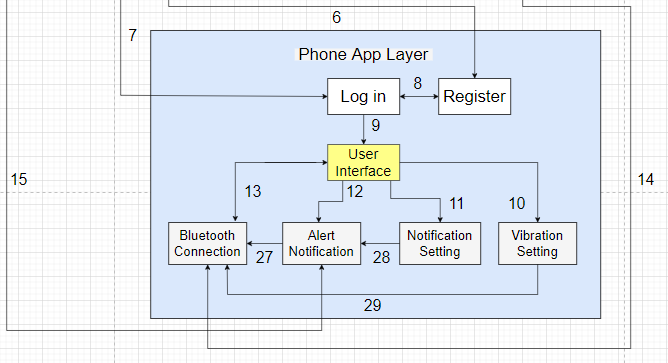
\includegraphics[width=0.60\textwidth]{images/phone_ui.png}
 \caption{Phone App Layer diagram}
\end{figure}

\subsubsection{Assumptions}
It is assumed that the user is already signed in.

\subsubsection{Responsibilities}
This subsystem is responsible for letting user to go to different settings and providing convenience to the user. 

\subsubsection{Subsystem Interfaces}
Each of the inputs and outputs for the subsystem are defined here. Create a table with an entry for each labelled interface that connects to this subsystem. For each entry, describe any incoming and outgoing data elements will pass through this interface.

\begin {table}[H]
\caption {User interfaces} 
\begin{center}
    \begin{tabular}{ | p{1cm} | p{6cm} | p{3cm} | p{3cm} |}
    \hline
    ID & Description & Inputs & Outputs \\ \hline
    #9 & From login & \pbox{User ID, password} & \pbox{Main page}  \\ \hline
    #13 & Bluetooth Connection & \pbox{Click on the 'Bluetooth' button} & \pbox{Bluetooth setting page}  \\ \hline
    #12 & Alert notification & \pbox{Click on the 'History' button} & \pbox{History list}  \\ \hline
    #11 & Notification setting & \pbox{Click on the 'Notification setting' button} & \pbox{Notification setting page}  \\ \hline
    #10 & Vibration setting & \pbox{Click on the 'Vibration setting' button} & \pbox{Vibration setting page}  \\ \hline
    \end{tabular}
\end{center}
\end{table}

\subsection{Bluetooth Connection}
The Bluetooth interface subsystem will allow users to turn on and off the Bluetooth communication and interact with the wristband module.

\begin{figure}[h!]
	\centering
 	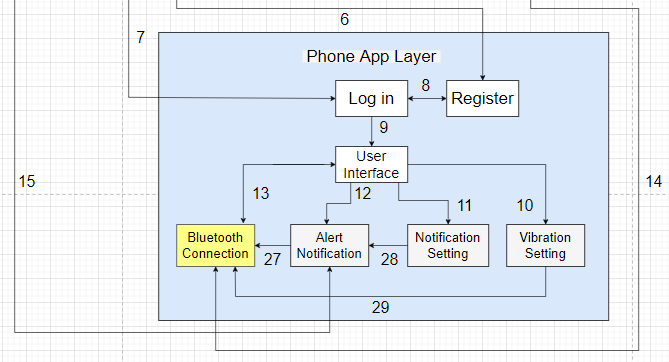
\includegraphics[width=0.60\textwidth]{images/phone_bluetooth.png}
 \caption{Phone App Layer diagram}
\end{figure}

\subsubsection{Assumptions}
It is assumed that the user is already signed in.

\subsubsection{Responsibilities}
This subsystem is responsible for letting users to set up Bluetooth and connect with their wristband module.

\subsubsection{Subsystem Interfaces}
Each of the inputs and outputs for the subsystem are defined here. Create a table with an entry for each labelled interface that connects to this subsystem. For each entry, describe any incoming and outgoing data elements will pass through this interface.

\begin {table}[H]
\caption {Bluetooth Settings interfaces} 
\begin{center}
    \begin{tabular}{ | p{1cm} | p{6cm} | p{3cm} | p{3cm} |}
    \hline
    ID & Description & Inputs & Outputs \\ \hline
    #29 & From vibration setting & \pbox{From vibration setting page} & \pbox{To Bluetooth setting}  \\ \hline
    #27 & From alert notification page & \pbox{From alert notification page} & \pbox{To Bluetooth setting}  \\ \hline
    #14 & Bluetooth setting & \pbox{Switch on and off} & \pbox{Bluetooth turns on and off}  \\ \hline
    #13 & To previous page & \pbox{Click on the back arrow} & \pbox{Main page}  \\ \hline
    \end{tabular}
\end{center}
\end{table}

\subsection{Alert notification}
The alert notification subsystem will allow users to view history on every past alert.

\begin{figure}[h!]
	\centering
 	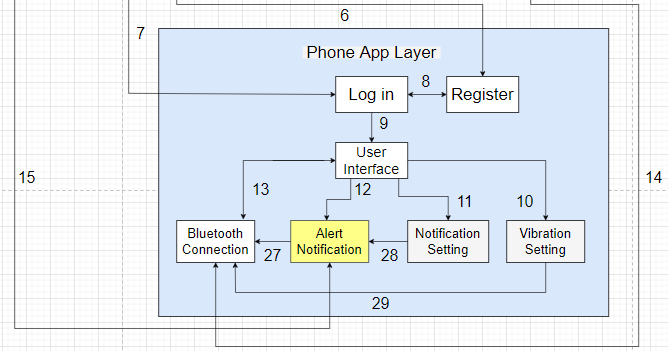
\includegraphics[width=0.60\textwidth]{images/phone_alert.png}
 \caption{Phone App Layer diagram}
\end{figure}

\subsubsection{Assumptions}
It is assumed that the user is already signed in.

\subsubsection{Responsibilities}
This subsystem will record and show all the past alerts on windows and doors. 

\subsubsection{Subsystem Interfaces}
Each of the inputs and outputs for the subsystem are defined here. Create a table with an entry for each labelled interface that connects to this subsystem. For each entry, describe any incoming and outgoing data elements will pass through this interface.

\begin {table}[H]
\caption {Alert notifications interfaces} 
\begin{center}
    \begin{tabular}{ | p{1cm} | p{6cm} | p{3cm} | p{3cm} |}
    \hline
    ID & Description & Inputs & Outputs \\ \hline
    #28 & From notification setting & \pbox{From notification setting} & \pbox{To alert notification}  \\ \hline
    #12 & To previous page & \pbox{Click on the back arrow} & \pbox{Main page}  \\ \hline
    #27 & To Bluetooth connection & \pbox{Click on the 'Bluetooth setting'} & \pbox{Bluetooth setting}  \\ \hline
    \end{tabular}
\end{center}
\end{table}

\subsection{Notification setting}
The notification setting interface subsystem will allow users to change settings for alarm notification.

\begin{figure}[h!]
	\centering
 	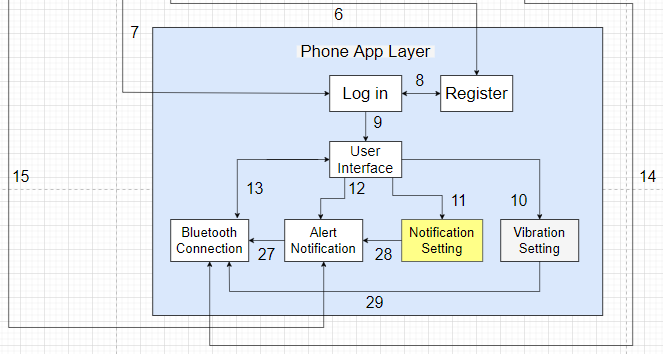
\includegraphics[width=0.60\textwidth]{images/phone_notification.png}
 \caption{Phone App Layer diagram}
\end{figure}

\subsubsection{Assumptions}
It is assumed that the user is already signed in.

\subsubsection{Responsibilities}
This subsystem will allow users to add or remove alerts for each window and the door.

\subsubsection{Subsystem Interfaces}
Each of the inputs and outputs for the subsystem are defined here. Create a table with an entry for each labelled interface that connects to this subsystem. For each entry, describe any incoming and outgoing data elements will pass through this interface.

\begin {table}[H]
\caption {Notification setting interfaces} 
\begin{center}
    \begin{tabular}{ | p{1cm} | p{6cm} | p{3cm} | p{3cm} |}
    \hline
    ID & Description & Inputs & Outputs \\ \hline
    #28 & Move to alert notification & \pbox{Click on the 'Alert notification'} & \pbox{Alert notification page}  \\ \hline
    #11 & To previous page & \pbox{Click on the back arrow} & \pbox{Main page}  \\ \hline
    \end{tabular}
\end{center}
\end{table}

\subsection{Vibration setting}
The notification setting interface subsystem will allow users to change vibration pattern as a notification.

\begin{figure}[h!]
	\centering
 	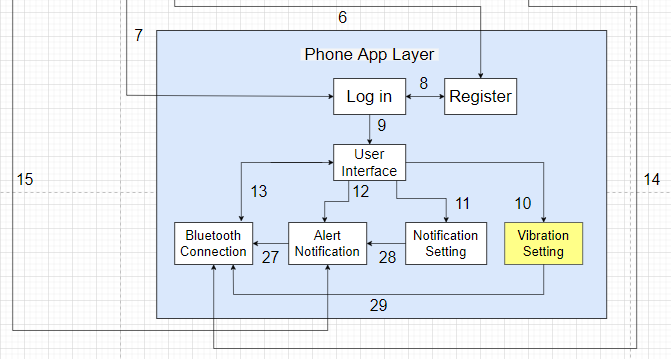
\includegraphics[width=0.60\textwidth]{images/phone_vibration.png}
 \caption{Phone App Layer diagram}
\end{figure}

\subsubsection{Assumptions}
It is assumed that the user is already signed in.

\subsubsection{Responsibilities}
This subsystem will allow users to change vibration patterns in a favor of users. For instance, the essential alert will vibrate stronger.

\subsubsection{Subsystem Interfaces}
Each of the inputs and outputs for the subsystem are defined here. Create a table with an entry for each labelled interface that connects to this subsystem. For each entry, describe any incoming and outgoing data elements will pass through this interface.

\begin {table}[H]
\caption {Vibration setting interfaces} 
\begin{center}
    \begin{tabular}{ | p{1cm} | p{6cm} | p{3cm} | p{3cm} |}
    \hline
    ID & Description & Inputs & Outputs \\ \hline
    #29 & Move to Bluetooth connection setting & \pbox{Click on 'Bluetooth'} & \pbox{Bluetooth page}  \\ \hline
    #10 & To previous page & \pbox{Click on the back arrow} & \pbox{Main page}  \\ \hline
    \end{tabular}
\end{center}
\end{table}
\newpage

%%% References
\bibliographystyle{plain}
\bibliographystyle{reference/IEEEtran_custom}
\bibliography{reference/refs}{}

\end{document}